% This is a LaTeX thesis template for Monash University.
% to be used with Rmarkdown
% This template was produced by Rob Hyndman
% Version: 6 September 2016

\documentclass{monashthesis}

%%%%%%%%%%%%%%%%%%%%%%%%%%%%%%%%%%%%%%%%%%%%%%%%%%%%%%%%%%%%%%%
% Add any LaTeX packages and other preamble here if required
%%%%%%%%%%%%%%%%%%%%%%%%%%%%%%%%%%%%%%%%%%%%%%%%%%%%%%%%%%%%%%%

\author{Xiefei Li}
\title{Revisiting the forecast combination puzzle: An empirical study}
\studentid{30204232}
\studentemail{\href{mailto:xlii0145@student.monash.edu}{\nolinkurl{xlii0145@student.monash.edu}}}
\studentdetails{Supervisor: David T. Frazier}
\supervisoremail{\href{mailto:David.frazier@monash.edu}{\nolinkurl{David.frazier@monash.edu}}}
\def\degreetitle{Bachelor of Commerce (Honours)}
% Add subject and keywords below
\hypersetup{
     %pdfsubject={The Subject},
     %pdfkeywords={Some Keywords},
     pdfauthor={Xiefei Li},
     pdftitle={Revisiting the forecast combination puzzle: An empirical study},
     pdfproducer={Bookdown with LaTeX}
}


\bibliography{thesisrefs}

\begin{document}

\pagenumbering{roman}

\titlepage

{\setstretch{1.2}\sf\tighttoc\doublespacing}

\clearpage\pagenumbering{arabic}\setcounter{page}{1}

\hypertarget{introduction}{%
\chapter{Introduction}\label{introduction}}

\hypertarget{research-objective}{%
\section{Research Objective}\label{research-objective}}

This thesis aims to investigate the determinants behind, and evidence for the forecast combination puzzle in various domains, and to empirically examine a general solution to the forecast combination puzzle. The combination puzzle refers to the well-known empirical finding that an equally weighted combination of forecasts generally outperforms more sophisticated combination schemes. This phenomenon is often found in the point combinations but it also appears in the density combinations. In this research, we will work with the density forecasts as point forecasts are implicitly included and they offer forecasters a more comprehensive view. Over the past 50 years, the empirical studies undertaken so far have focused more on different time series settings. Thus, one of the main contributions of this research will be to investigate the presence of the combination puzzle in settings outside of pure time series models with density forecasts. As an additional contribution, we will assess the veracity, and applicability, of a recently proposed solution to the forecast combination puzzle suggested in \textcite{ZMFP22} and \textcite{FZMP23}.

\hypertarget{literature-review-and-motivation}{%
\section{Literature Review and Motivation}\label{literature-review-and-motivation}}

The accuracy of forecasts is of critical concern for forecasters and decision makers. An idea of combining multiple forecasts from different models was originally proposed in the seminal work of \textcite{BG69}. With the evidence of dramatic improvements in the forecast accuracy, forecast combinations have attracted increasing attention and contributions in the literature, both theoretical and applied \autocite{C89,T06}. In short, forecast combination methods involve producing point or density forecasts and then combining them based on a rule or weighting scheme. This process can sometimes capture more meaningful characteristics of the true data generating process than using a single model, and allow us to combine the best features of different models within a single framework. Researchers have examined a variety of combination methods for both point and density forecasts over the past 50 years, see \textcite{WHLK22} for a modern literature review.

In most time series setting under which forecast combinations are employed, a striking empirical phenomenon is often observed, coined by \textcite{SW04}, as the ``forecast combination puzzle''. The puzzle is encapsulated by the fact that ``theoretically sophisticated weighting schemes should provide more benefits than the sample average from forecast combination, while empirically the simple average has been continuously found to dominate more complicated approaches to combining forecasts'' \autocite{WHLK22}. In the literature, there are two possible explanations for the puzzle. One concentrates on the estimation uncertainty in combination weight (\textcite{SW98}, \textcite{SW04} and \textcite{SW09}). Complicated weighting schemes introduce variability when estimating parameters whereas the simple averaging does not require any estimation. On the other hand, \textcite{E11} and \textcite{CMVW16} explore the trade-off between bias and variance in the Mean Squared Forecast Error (MSFE). They proved that equally weighted combination is unbiased and its variance has only one component, resulting in a smaller mean squared error than a biased combination. However, this is mainly applicable to the MSFE scheme. Recently, \textcite{ZMFP22} and \textcite{FZMP23} proposed a new explanation for the puzzle in a general way by investigating the sampling variability of the forecasts induced via estimation of the constituent model forecasts (i.e., the models used to produce the forecasts). They illustrated that, asymptotically, the bias and variability mainly come from the estimation of the models used to produce the constituent model forecasts.

The goal of this thesis is two-fold: first, to search for empirical evidence of the combination puzzle in settings outside of the usual time series in which it has been found; second, to test the empirical veracity of the theoretical solution to the puzzle found in \textcite{FZMP23}, both within, and outside of, the standard time series setting where the puzzle is often observed.

\hypertarget{methodology}{%
\chapter{Methodology}\label{methodology}}

The first goal of this paper is to construct linear density forecast combinations with parametric models. The results are anticipated to reveal that forecast combinations can deliver improved accuracy over single models, but are not necessarily superior to forecasts obtained from the equally weighted combination.

The next goal is to estimate the unknown parameters of the constituent models and the weight in a single step, and to compare the accuracy of forecasts based on these combinations against the usual combinations process, as well as the equally weighted combination. To measure differences between these forecasts, we will eventually employ forecast accuracy tests, of the type derived in \textcite{W96}, which measure out-of-sample differences between forecasts.

Before explaining further details, the following notation will be used throughout the paper. A vector time series \(\textbf{y}_t\) with a total of \(T\) observations will be divided proportionally into two parts, an in-sample period \(R\) and an out-of-sample period \(P\). The realization of a target variable \(y\) at time \(t\) is denoted as \(y_{t}\). Its future values after the in-sample period is denoted as \(y_{\small{R+h}}\), where \(h\) is the forecast horizon and \(h>0\). The information set at time t, \(\mathcal{F}_t\), is comprised of all observed (and known) realizations of \(y\) up to time t, i.e., \(\mathcal{F}_t = \{y_1, y_2, .., y_t\}\).

A prediction model \(M\) determines the conditional probability density for \(\textbf{y}_t\) with unknown parameters \(\theta_M\) given the history \(\mathcal{F}_{t-1}\), denoted by \(f(y_t|\mathcal{F}_{t-1}, \theta_M, M)\). Parameter estimates \(\hat\theta_M\) are obtained by maximizing the log likelihood function of the conditional probability density for the in-sample period, i.e., \(\hat\theta_M = \text{argmax} \sum^R_{t=1} log f(y_t|\mathcal{F}_{t-1}, M)\). These estimates will be held fixed for the ease of evaluation.

\hypertarget{forecast-combination-linear-pools}{%
\section{Forecast Combination: Linear Pools}\label{forecast-combination-linear-pools}}

Based on the idea of linear pooling \autocite{BG69,HM07,GA11}, a linear combination of two densities \(f(y_t)\) is constructed with two constituent densities \(f_1(y_t)\) and \(f_2(y_t)\):

\begin{equation}
f(y_t) = wf_1(y_t) + (1-w)f_2(y_t)
\end{equation}

where \(w\) is the weight allocated to the first density. Through this construction, the sum of two weights is implied to be 1, which is necessary and sufficient for the combination to be a density function \autocite{GA11}.

The optimal weight will be estimated by maximizing the log score function over the in-sample period for all possible sets of the two-model linear combination.

\begin{equation}
\hat{w}_{\text{optimal}} = \text{argmax} \sum^R_{t=1}log \Big[w \ f_1(y_t |\mathcal{F}_{\small{t-1}}, \hat\theta_1) + (1-w) \ f_2(y_t|\mathcal{F}_{\small{t-1}}, \hat\theta_2)\Big] 
\end{equation}

Following the literature on density forecast evaluation, our initial analysis will focus on using log predictive score functions to measure the accuracy of our density forecasts; see, e.g., \textcite{GA11} for a discussion on log score and its use in density forecasting. The log predictive score function for a linear combination of two predictive densities over the forecast horizon \(h=1,2,...,P\) (i.e., the out-of-sample period) is defined as follows:

\begin{equation}
\label{eqn:LS}
LS = \sum^P_{h=1} log \Big[ \hat{w}_{\text{optimal}} f_1(y_{\small{R+h}}| \mathcal{F}_{\small{R+h-1}}, \hat\theta_1) + (1-\hat{w}_{\text{optimal}}) \ f_2(y_{\small{R+h}}| \mathcal{F}_{\small{R+h-1}}, \hat\theta_2)\Big].
\end{equation}

\hypertarget{preliminary-results}{%
\chapter{Preliminary Results}\label{preliminary-results}}

\hypertarget{a-motivating-example}{%
\section{A Motivating Example}\label{a-motivating-example}}

Reconsidering the example in section 3 of \textcite{GA11}, the data we use is the daily Standard and Poor's (S\&P) 500 index from February 11, 2013 to February 10, 2023 (10 years in total), retrieved from the \textcite{SP500}. We choose \(j=1,\cdots,M\), with \(M=5\) prediction models to study the performance of density predictions across sets of \texttt{two-model} pools. Each of the \(j\) predictive model has a conditional Gaussian density, which takes the form \(f^{(j)}(y)=f_j(y_t|\mathcal{F}_{t-1})=N\{y_t; \mu_j, \sigma^2_j\}\), where \(N\{x; \mu, \sigma^2\}\) denotes the normal probability density function evaluated at value \(x\) with mean \(\mu\) and variance \(\sigma^2\). The notation \(\mathcal{F}_{t-1}\) denotes all information available at time \(t-1\), and we assume that the conditional mean and variance of the models are, up to unknown parameters, known at time \(t-1\).

Candidate models include commonly used model types such as autoregressive integrated moving average (ARIMA), exponential smoothing (ETS), and linear regression model with ARIMA errors. See the Appendix for detailed model specifications.

\begin{table}[ht]
  \centering
  \caption{Log predictive score of density forecasts combination under two-model pools}
    \begin{tabular}{llllll}
    \toprule
          & ARIMA(1,1,1) & ETS(M,N,N) & ETS(M,A,N) &  LM (linear) &  LM (log) \\
    \midrule
    ARIMA(1,1,1) & \textit{-5911.1974} & -5839.3045 & -5842.7634 & -5911.1974 & -5894.1267 \\
    ETS(M,N,N) & 0.45  & \textit{-5883.9697} & -5881.7790 & -5883.9697 & -5858.6397 \\
    ETS(M,A,N) & 0.43  & 0.08  & \textit{-5881.7970} & -5881.7970 & -5859.7980 \\
     LM (linear) & 1     & 1     & 1     & \textit{-7532.1464} & -5918.5230 \\
     LM (log) & 0.56  & 0.65  & 0.67  & 0     & \textit{-5918.5230} \\
    \bottomrule
    \multicolumn{6}{l}{\footnotesize The diagonal entries contains individual log score.}\\
    \multicolumn{6}{l}{\footnotesize The log scores for combination pools are located above the diagonal.}\\
    \multicolumn{6}{l}{\footnotesize Entries below diagonal show the estimated weight of the model in that column in the two-model pool.}\\
    \end{tabular}
  \label{tab:2}
\end{table}

There are 10 sets of two-model combination and the log predictive score of each combination is generated according to \ref{eqn:LS} with the value of weight changing by 0.01 every time. Table \ref{tab:2} shows the estimated weights and combination log scores.

\vspace{0.3cm}

\begin{figure}[ht]
\centering
\caption{The highest four log predictive scores of weighted two-model combinations for S\&P 500 index predictive densities.}
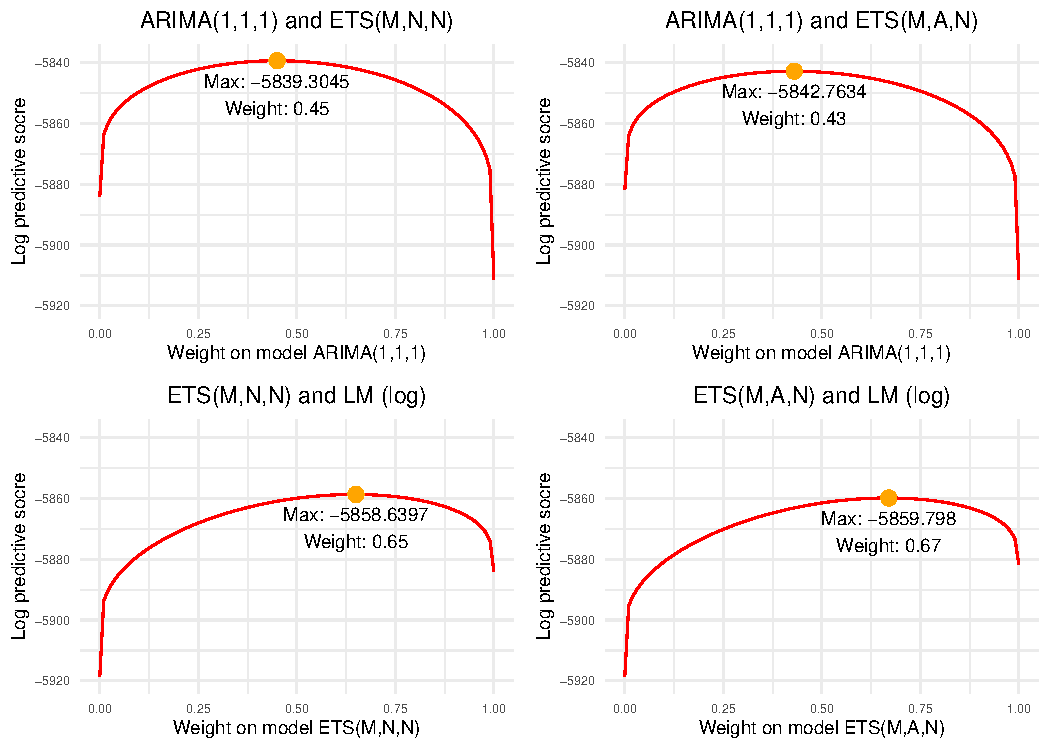
\includegraphics{figures/best4comb.pdf}
\begin{flushleft}
{\footnotesize The weights on the first model is in the x-axis and the corresponding log predictive scores are on the y-axis. Constituent models are stated in the title. The orange point represent the highest log score of a specific combination. Its value and the corresponding estimated weight are noted below.}\\
\end{flushleft}
\label{fig:best4}
\end{figure}

Figure \ref{fig:best4} illustrates the change of the log predictive score for the top 4 combinations as the weight increases. The great improvements in all scores mean that combination forecasts do perform better than the individual forecasts. It is also noticeable that the estimated weightis ``close to'' the equal-weighted benchmark, which could be an evidence for the forecast combination puzzle.

We have shown that the forecast combination puzzle is evident in the time series setting. We will then exploit the puzzle more extensively with the panel data in the next chapter.

\hypertarget{timeline-of-future-research}{%
\section{Timeline of Future Research}\label{timeline-of-future-research}}

\begin{table}[htbp]
  \centering
  \caption{Research Plan}
    \begin{tabular}{ll}
    Time  & Objectives \\
    \midrule
    May - June & Investigating the presence of puzzle in panel data and literature review \\
    July - August & Applying forecast accuracy tests with time series data and drafting thesis  \\
    September & Applying tests with panel data and considering limitations \\
    October & Working on thesis and final presentation \\
    \end{tabular}
\end{table}

\appendix

\hypertarget{appendix}{%
\chapter{Appendix}\label{appendix}}

The S\&P500 index dataset has a total of 2519 (\(T\)) observations and is partitioned into two periods with a rough proportion. The in-sample period contains the first 60\% of the data (\(R = 1511\)), which is used to estimate all unknown parameters, including the optimal weight. The remaining 40\% (\(P = 1008\)) becomes the out-of-sample period to evaluate the forecast performance.

The following predictive models are used to study the two-model pools:

\begin{enumerate}
\def\labelenumi{\arabic{enumi}.}
\item
  Model 1: ARIMA(1,1,1) model with an intercept of the natural logarithm of S\&P 500 index.
  \begin{equation*}
  log(y_t) = c + log(y_{t-1}) + \phi_1\big[log(y_{t-1})-log(y_{t-2})\big] + \epsilon_t + \theta_1\epsilon_{t-1}
  \end{equation*}
\item
  Model 2: ETS(M,N,N) model of the S\&P 500 index.
  \begin{align*}
  y_t &= \ell_{t-1} (1+\epsilon_t) \\
  \ell_t &= \ell_{t-1} (1+\alpha \epsilon_t) \\
  \end{align*}
\item
  Model 3: ETS(M,A,N) model of the S\&P 500 index.
  \begin{align*}
  y_t &= (\ell_{t-1} + b_{t-1})(1+\epsilon_t) \\
  \ell_t &= (\ell_{t-1} + b_{t-1}) (1+\alpha \epsilon_t) \\
  b_t &= b_{t-1} + \beta (\ell_{t-1} + b_{t-1})\epsilon_t \\
  \end{align*}
\item
  Model 4: A linear regression model of the S\&P 500 index and ARIMA(1,0,0) errors.
  \begin{align*}
  y_t &= \beta_0 + \beta_1 t + u_t \\
  u_t &= \phi_1 \epsilon_{t-1} + \epsilon_t
  \end{align*}
\item
  Model 5: A linear regression model of the natural logarithm of the S\&P 500 index and ARIMA(1,0,0) errors.
  \begin{align*}
  log(y_t) &= \beta_0 + \beta_1 t + u_t \\
  u_t &= \phi_1 \epsilon_{t-1} + \epsilon_t
  \end{align*}
\end{enumerate}

The \(\epsilon_t\) in each model is assumed to be independent and normally distributed with a zero mean and a constant variance.

Exact formulas and explanations of these models can be found in \textcite{fpp3}. The formula of the conditional variance for the ETS models in this case is discussed in Chapter 6.3 of \textcite{HKOS08}. All codes are performed in R Statistical Software (version 4.2.1 (2022-06-23)). The packages used are \texttt{tidyverse} \autocite{tidy19}, \texttt{dplyr} \autocite{dplyr23}, and \texttt{fpp3} \autocite{fpp23}.

The unknown parameters are estimated by maximizing the likelihood function using the in-sample period data. Once the estimated are obtained, they are held fixed for the density evaluation. For each model, we generate the predictive densities at every future time point of S\&P 500 index (\(h=1,2,...,P\)) given that all past information is known. In order to make a comparison between models, the log of S\&P 500 index will be evaluated by the log normal density function.

The log predictive score of each model is calculated and presented in Table \ref{tab:1}. If only one model can be chosen, the model with the highest score will be preferred, which is the ETS(M,A,N) model with a score of -5881.7970 in this case.

\vspace{0.3cm}

\begin{table}[htbp!]
\centering
\caption{Log score of each candidate model}
\begin{tabular}{l*{4}{c}cccccccc}
\hline
     ARIMA(1,1,1) & ETS(M,N,N) & ETS(M,A,N) & LM (linear) & LM (log) \\
    \hline
     -5911.1974 & -5883.9697  & -5881.7970 & -7532.1464 & -5918.5230\\
    \hline
\end{tabular}
\label{tab:1}
\end{table}

The top 4 combinations and their log scores are collected in Table \ref{tab:3}.

\begin{table}[ht]
  \centering
  \caption{The top four density forecast combinations evaluated by the log predictive score function}
    \begin{tabular}{ll}
    \toprule
    Combination & Log predictive score \\
    \midrule
    ARIMA(1,1,1) and ETS(M,N,N) & -5839.3045 \\
    ARIMA(1,1,1) and ETS(M,A,N) & -5842.7634 \\
    ETS(M,N,N) and  LM (log) & -5858.6397 \\
    ETS(M,A,N) and  LM (log) & -5859.7980 \\
    \bottomrule
    \end{tabular}
  \label{tab:3}
\end{table}

\printbibliography[title={Reference}]




\end{document}
